\documentclass{article}
\usepackage{amsmath}
\usepackage{graphicx}

\newcommand{\biggbreak}{\\[1ex]}

\title{Q2}
\author{qwrx21}

\begin{document}
\maketitle
\pagebreak

\subsection*{Initial Table}

\begin{center}
\begin{tabular}{c|c c c c c c}
    
    &A&B&C&D&E&F \\
    \hline
    A&0&\underline{15}&24&29&25&37 \\
    B&15&0&32&31&23&43 \\
    C&24&32&0&30&43&49 \\
    D&29&31&30&0&45&57 \\
    E&25&23&43&45&0&55 \\
    F&37&43&49&57&55&0 \\
    
\end{tabular}
\end{center}


\subsection*{1st reduction}

\begin{center}
\begin{tabular}{c|c c c c c c}
    
    & $Z_2$ &C&D&E&F \\
    \hline
    $Z_2$&0&28&30&\underline{24}&40 \\
    C&28&0&30&43&49 \\
    D&30&30&0&45&57 \\
    E&24&43&45&0&55 \\
    F&40&49&57&55&0 \\
   
    
\end{tabular}
\end{center}

\subsection*{2nd reduction}

\begin{center}
\begin{tabular}{c|c c c c c c}
    
    & $Y_3$ &C&D&F \\
    \hline
    $Y_3$&0&33&35&45 \\
    C&33&0&\underline{30}&49 \\
    D&35&30&0&57 \\
    F&45&49&57&0 \\
   
    
\end{tabular}
\end{center}

\subsection*{3rd reduction}

\begin{center}
\begin{tabular}{c|c c c c c c}
    
    & $Y_3$ &$X_2$&F \\
    \hline
    $Y_3$&0&\underline{34}&45 \\
    $X_2$&34&0&53 \\
    F&45&53&0 \\
   
    
\end{tabular}
\end{center}

\subsection*{4th reduction}

\begin{center}
\begin{tabular}{c|c c}
    
    & $W_5$ &F \\
    \hline
    $W_5$&0&48.2 \\
    F&48.2&0 \\
   
    
\end{tabular}
\end{center}
\subsection*{Tree}
\begin{figure}
    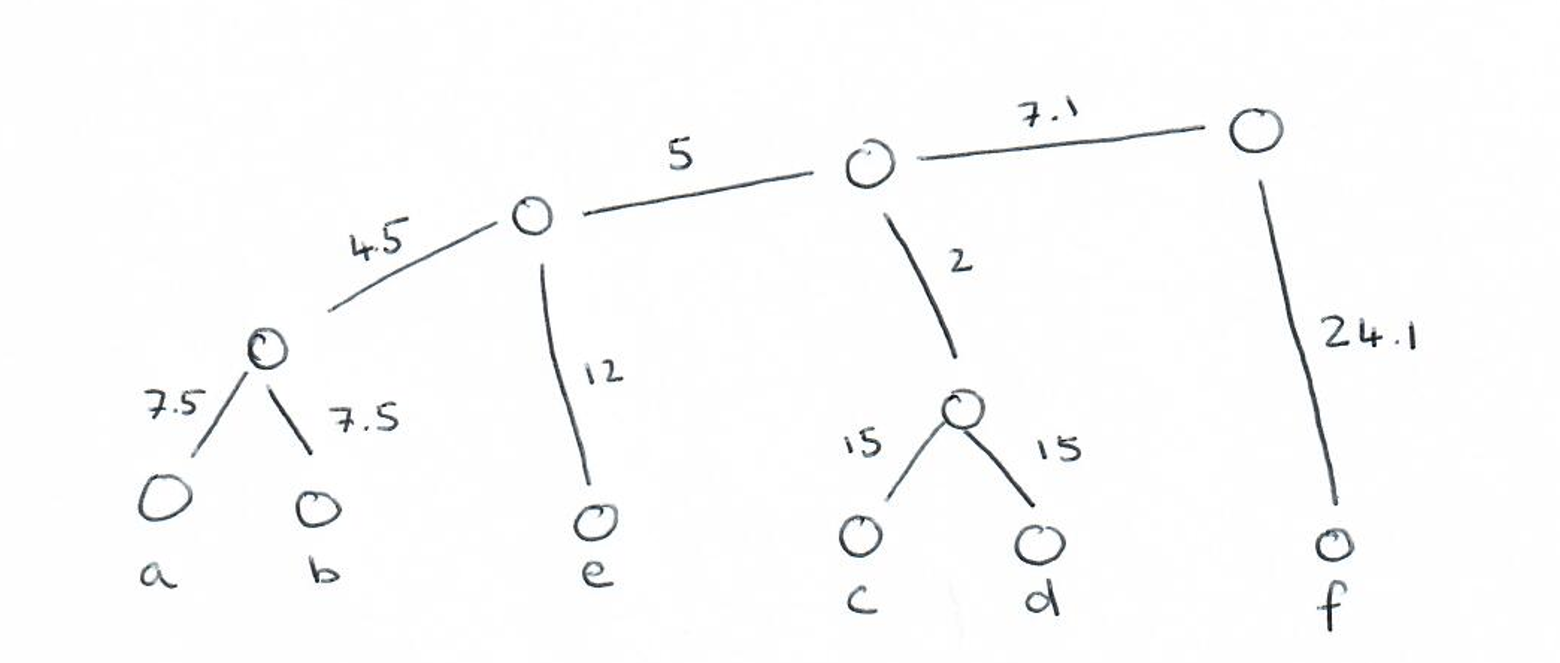
\includegraphics[width=\linewidth]{Tree.png}
    \caption{Tree}
    \label{fig:boat1}
  \end{figure}
  




\end{document}


